\chapter{Anexo}

\section{Demostración Ley de Walras}

Definimos el exceso de demanda como $\textit{q}(p)$ (ecuación \ref{eq: e demand}) considerando las demandas marshallianas de los bienes $x$ e $y$ y las dotaciones $\omega_x$ y $\omega_y$. Por notación dejamos las demandas marshallianas como $\xi_j$ siendo $j$ el conjunto de bienes, esto con el fin de generalizar la ecuación. 
\begin{equation}
     \textit{q}(p) =  \left[  \sum ^n _{j} \xi_j - \sum ^n _{j} \omega_j \right] \label{eq: e demand}
\end{equation}

Donde además diremos que para todo mercado $j$ se cumple la igualdad.
\begin{equation}
    \sum ^n _{j} p_j \xi _j(p,R) = \sum ^n _{j} p_j \omega_j \label{eq: eq de mercado}
\end{equation}

Para completar la demostración ponderamos el exceso de demanda por el vector $p$.
\begin{equation}
    p\textit{q}(p) = p \left[  \sum ^n _{j} \xi_j - \sum ^n _{j} \omega_j \right] = \sum ^n _{j} \left[ p_j \xi_j(p,R) - p_j \omega_j    \right] = 0
\end{equation}

Lo cual se debiera cumplir por la igualdad (\ref{eq: eq de mercado}). 


\section{Equilibrio General con Producción}

Una extensión de lo visto en el modelo de equilibrio general con dos bienes y dos agentes sería considerar los factores productivos y funciones de producción con los que se crean los bienes. En este caso las dotaciones no van a ser de bienes sino de factores de producción capital y trabajo ($K,L$). Habrá un total de capital de $\bar{K}$ y un total de trabajo $\bar{L}$, con los que se producen los bienes $x,y$. 

Análogo al consumo la condición de eficiencia para la producción sigue siendo la igualdad entre las tasas marginales, en este caso la \textbf{tasa marginal técnica} (TMT) de sustitución. Es decir, la producción de un bien que podemos intercambiar por la producción adicional de una unidad del otro,
\begin{equation}
    TMT = \frac{ \frac{\partial f(K,L)}{\partial K} }{\frac{\partial f(K,L)}{\partial L} } \label{eq: TMT dfn}
\end{equation}
Dado que se requieren capital y trabajo para los dos bienes estos se tendrán que repartir las dotaciones de manera eficiente, siguiendo \ref{eq: TMT = TMT}.
\begin{equation}
    TMT^x_{K,L} = TMT^y_{K,L} \label{eq: TMT = TMT}
\end{equation}
Podemos formar una caja de Edgeworth de producción como se puede ver en la figura \ref{fig:diapositiva4}.
\begin{figure}[htbp]
    \centering
    \caption{Caja de Edgeworth en la producción}
    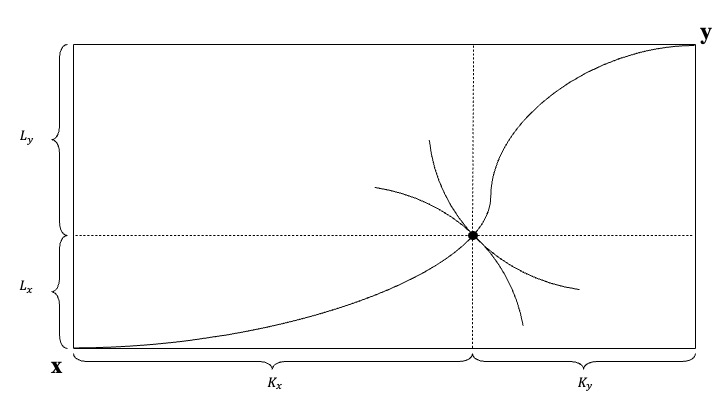
\includegraphics[width=\textwidth]{Figuras/EG Curva de contrato con produccion.jpeg}
    \label{fig:diapositiva4}
\end{figure}
Las curvas de contrato se relacionan con las fronteras de posibilidades. La \textbf{frontera de posibilidades}\marginnote{\textbf{Frontera de posibilidades:}} es una curva que describe todos los puntos en donde se ocupan eficientemente los factores productivos para producir dos bienes, es decir, son los puntos factibles donde no es posible aumentar la producción de un bien sin disminuir la producción del otro. En la figura \ref{fig:diapositiva5} se observan dos puntos, uno que está ubicado en la curva es eficiente y otro que no es eficiente puesto que se puede producir más de un bien sin disminuir la producción de otro. Como todos los puntos de la curva de contrato satisfacen la condición de eficiencia se puede decir que también pertenecen a la curva de contrato.
\begin{figure}[htbp]
    \centering
    \caption{Frontera de posibilidades de producción}
    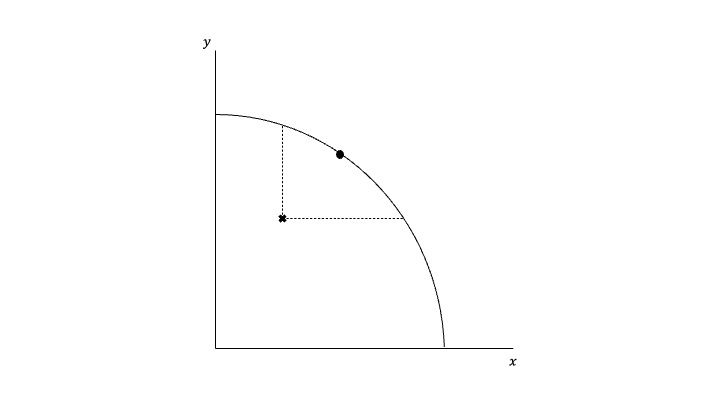
\includegraphics[width=\textwidth]{Figuras/EQ Frontera de posibilidades de produccion.jpeg}
    \label{fig:diapositiva5}
\end{figure}

Para resolver el modelo: Habrá una dotación de factores productivos $K,L$ en donde habrá un total de $\bar{K}$ y $\bar{L}$ para cada factor respectivamente. Asumiremos la función Cobb-Douglas para la función de utilidad y de producción.  
\begin{align*}
    U_i (x_i,y_i) = x_i^\alpha y_i ^{1-\alpha},  \quad i = A,B \\
    x(K,L) = K_x^\beta L_x ^{1-\beta}, \quad y(K,L) = K_y^\beta L_y^{1-\beta}  
\end{align*}
Es decir que los dos individuos consumen los bienes $x,y$ producidos con los factores $K,L$. Las variables $\alpha$ y $\beta$ representan las preferencias y ponderaciones para el consumo y producción respectivamente. 

\subsubsection*{Curva de contrato de producción}

La eficiencia de producción se dará maximizando la producción de un bien sujeta a la producción del otro. De esta manera encontraremos los puntos que pertenecen a la frontera de posibilidades y que por tanto son eficientes. 
\begin{align*}
    \max _{K_x,L_x} \quad &x = K_x^\beta L_x^{1-\beta}\\
    \text{s.a} \quad  y =& K_y^\beta L_y^{1-\beta} \\
     \Bar{K} =& K_x + K_y \\
     \Bar{L} =& L_x + L_y
\end{align*}

Planteando el lagrangeano y resolviendo podemos optimizar la funcíon.
\begin{equation*}
    \mathcal{L}: \quad K_x^\beta L_x^{1-\beta} + \lambda_1(K_y^\beta L_y^{1-\beta} - y) + \lambda_2(K_x + K_y - \Bar{K}) + \lambda_3(L_x + L_y - \Bar{L}) 
\end{equation*}
Encontramos las condiciones de primer orden.
\begin{align}
    \frac{\partial \mathcal{L}}{\partial K_x} &= \beta K_x^{\beta-1}L_x^{1-\beta} + \lambda_2 = 0 \\ 
    \frac{\partial \mathcal{L}}{\partial L_x} &= (1-\beta)K_x^\beta L_x^{-\beta} + \lambda_3 = 0 \\
    \frac{\partial \mathcal{L}}{\partial K_y} &= \lambda_1\beta K_y^{\beta-1}L_y^{1- \beta} + \lambda_2 = 0 \\
    \frac{\partial \mathcal{L}}{\partial L_y} &= \lambda_1 (1-\beta) K_y^\beta L_y^{-\beta} + \lambda_3 = 0
\end{align}
De las condiciones de primer orden encontramos las tasas marginales técnicas parala producción de los dos bienes. Despejando y dividiendo las expresiones para cada producto.
\begin{align}
    \frac{\beta K_x^{\beta-1}L_x^{1-\beta}}{(1-\beta)K_x^\beta L_x^{-\beta}} = \frac{-\lambda_2}{-\lambda_3} \Longrightarrow \left( \frac{\beta}{1-\beta} \right)\frac{L_x}{K_x} = \frac{\lambda_2}{\lambda_3} \\
    \frac{\lambda_1\beta K_y^{\beta-1}L_y^{1- \beta}}{\lambda_1 (1-\beta) K_y^\beta L_y^{-\beta}} = \frac{-\lambda_2}{-\lambda_3} \Longrightarrow \left( \frac{\beta}{1-\beta} \right) \frac{L_y}{K_y} = \frac{\lambda_2}{\lambda_3}
\end{align}
Como condición de eficiencia las tasas marginales de transformación deben ser iguales para los dos bienes. Al igualar encontraremos la curva de contrato de producción, es decir, los puntos eficientes para la producción. 
\begin{equation}
    \frac{L_x}{K_x} = \frac{L_y}{K_y}
\end{equation}
La curva de contrato es bastante simple en este caso pues asumimos que los dos bienes se producen de la misma manera $x(K,L) = y(K,L)$. Considerando los totales de producción podemos reescribir la expresión llegando a \ref{eq: curva de contrato para la producción},
\begin{align}
    \frac{L_x}{K_x} &= \frac{\bar{L}-L_x}{\bar{K}-K_x} \notag \\
    K_x = \frac{\bar{K}}{\bar{L}}L_x &\Longleftrightarrow K_y = \frac{\bar{K}}{\bar{L}}L_y   \label{eq: curva de contrato para la producción}
\end{align}

\subsubsection*{Frontera de posibilidades de producción}
Para obtener la frontera de posibilidades utilizamos la expresión \ref{eq: curva de contrato para la producción} para obtener la cantidad óptima de factores para producir $x$ e $y$. 
\begin{align*}
    x(K,L) = K_x^\beta L_x^{1-\beta}, \quad K_x = \frac{\bar{K}}{\bar{L}}L_x \\
    x = \left( \frac{\bar{K}}{\bar{L}}L_x \right)^\beta L_x^{1-\beta} = \left( \frac{\bar{K}}{\bar{L}} \right)^\beta L_x \\
    L_x =  \frac{\bar{L}^\beta}{\bar{K}^\beta}  x
\end{align*}
Reemplazando de vuelta en \ref{eq: curva de contrato para la producción} obtenemos,
\begin{align}
    L^*_x =  \frac{\bar{L}^\beta}{\bar{K}^\beta}  x \Longleftrightarrow K^*_x = \frac{\bar{K}^{1-\beta}}{\bar{L}^{1-\beta}}  x
\end{align}
Como el problema es simétrico sería lo mismo para la produccióndel bien $y$. 
\begin{align*}
    L^*_y =  \frac{\bar{L}^\beta}{\bar{K}^\beta} y \Longleftrightarrow K^*_y = \frac{\bar{K}^{1-\beta}}{\bar{L}^{1-\beta}}  y
\end{align*}
Ahora que tenemos la cantidad óptimo de factores para un mismo bien podemos utilizar las expresiones para encontrar la frontera de posibilidades de producción. 
\begin{align*}
    L^*_x + L_y^* = \bar{L} \\
    \frac{\bar{L}^\beta}{\bar{K}^\beta}y + \frac{\bar{L}^\beta}{\bar{K}^\beta}x = \bar{L} \\
    \frac{\bar{L}^\beta}{\bar{K}^\beta}y = \bar{L} -  \frac{\bar{L}^\beta}{\bar{K}^\beta}x \\
    \text{FPP:} \quad y = \left( \frac{\bar{K}}{\bar{L}} \right)^\beta - x 
\end{align*}

La pendiente es lineal es igual a $1$, esto porque simplificamos bastante al plantear las producciones y el consumo.

\subsubsection*{Curva de contrato del consumo}

Al igual que antes planteamos el problema con las restricciones correspondientes, ahora, con la restricción de la frontera de posibilidades.
\begin{align*}
    \max _{x_A,y_A} \quad & U_A = x_A^\alpha y_A^{1-\alpha} \\
    \text{s.a} \quad  U_B&= x_B^\alpha y_B^{1-\alpha} \\
     \bar{x} &= x_A + x_B \\
    \bar{y} &= y_A + y_B \\
    \bar{y} &= \left( \frac{\bar{K}}{\bar{L}} \right)^\beta - x 
\end{align*}
Planteamos el lagrangeano
\begin{align*}
    \mathcal{L}:\quad x_A^\alpha y_A^{1-\alpha} + \lambda_1 (x_B^\alpha y_B^{1-\alpha} - U_B) + \lambda_2 (x_A + x_B - \bar{x}) + \\ \lambda_3 (y_A + y_B - \bar{y}) + \lambda_4 \left( \left( \frac{\bar{K}}{\bar{L}} \right)^\beta - \bar{x} - \bar{y} \right)
\end{align*}
Derivamos para obtener las condiciones de primer orden. 
\begin{align}
    \frac{\partial \mathcal{L}}{\partial x_A} &= \alpha x_A^{\alpha - 1}y_A^{1- \alpha} + \lambda_2 = 0 \\
    \frac{\partial \mathcal{L}}{\partial y_A} &= (1-\alpha)x_A^\alpha y_A^{-\alpha} + \lambda_3 = 0 \\
    \frac{\partial \mathcal{L}}{\partial x_B} &= \lambda_1\alpha x_B ^{\alpha - 1}y_B ^{1-\alpha} + \lambda_2 = 0 \\
    \frac{\partial \mathcal{L}}{\partial y_B} &= \lambda_1(1-\alpha) x_B^{\alpha} y_B^{-\alpha} + \lambda_3 = 0 \\
    \frac{\partial \mathcal{L}}{\partial \bar{x}} &= - \lambda_2 - \lambda_4 = 0 \\
    \frac{\partial \mathcal{L}}{\partial \bar{y}} &= - \lambda_3 - \lambda_4 = 0
\end{align}

Resolvemos sistemáticamente para obtener las tasas de sustitución de los bienes para cada individuo y en este caso consideramos la frontera de posibilidades.
\begin{align}
    \frac{\alpha x_A^{\alpha - 1}y_A^{1- \alpha}}{(1-\alpha)x_A^\alpha y_A^{-\alpha}}  = \frac{-\lambda_2}{-\lambda_3} \Longrightarrow \left( \frac{\alpha}{1-\alpha} \right) \frac{y_A}{x_A} = \frac{\lambda_2}{\lambda_3} \\
    \frac{\lambda_1\alpha x_B ^{\alpha - 1}y_B ^{1-\alpha} }{\lambda_1(1-\alpha) x_B^{\alpha} y_B^{-\alpha} } = \frac{-\lambda_2}{-\lambda_3} \Longrightarrow \left( \frac{\alpha}{1-\alpha} \right) \frac{y_B}{x_A} = \frac{\lambda_2}{\lambda_3} \\
    \frac{-\lambda_2}{-\lambda_3} = \frac{\lambda_4}{\lambda_4} \Longrightarrow \frac{\lambda_2}{\lambda_3} = 1
\end{align}
Acabamos de ver como la pendiente en el consumo coincide con la pendiente de la frontera de posibilidades. Cuadró la eficiencia en la producción de los bienes como en el consumo de los mismos.

Para ver este mismo proceso y ejercitar puede ver el siguiente video \href{https://youtu.be/NgxHDSLMPbo?si=6epG7OJTwx6sANFj}{\underline{link}}.


\section{Soluciones a la Coase}
% no me acuerdo de donde habré sacado este ejercicio.
Un ejemplo de como se plantea la solución a la Coase mediante la maximización de utilidad y los óptimos de pareto. Dos compañeros de piso Agustín ($A$) y Benjamín ($B$) tienen un problema de externalidades, Agustín le gusta fumar y Benjamín detesta el olor a cigarro. 

En esta economía solo exiten dos bienes, los cigarros $c$ los cuales emiten una polución $s$ y un bien genérico $x$. La utilidad de $A$ se puede denotar como $U_A (x_A,c_A)$ siendo el efecto marginal de estos dos bienes positivos. Además, $A$ tiene que respetar un máximo de polución $s_M (c_M)$, es decir, no se puede fumar más de $c_M$ cigarros. El precio del bien $x$ es numerario. Benjamín por su parte tendrá una función de utilidad $U_B(x_B, c_A) = u(x_B) + d(s_B)$ en la cual $u'(x_B) >0$ y $d'(s_B)<0$. Las dotaciones iniciales de cada uno son $\omega_A (X_A,\bar{c})$ y $\omega_B = (X_B,0)$. 

Dadas estas condiciones no habrá un resultado eficiente. Agustín fuma lo máximo que se le permite $c_A = c_M$ causando una polución $s_M$ sin internalizar el daño $d_B(s_M)$ hecho a Benjamín. Lo anterior causa que las tasas marginales difieran pues no se internalizan todos los costos, llevando a un resultado ineficiente.\footnote{Hay casos en que aun habiendo externalidades no se modifica el resultado eficiente, estos es por ejemplo cuando} 
% Desarrollar idea
\begin{equation}
    \frac{\frac{\partial U_A(x_A,c_A)}{\partial x_A}}{\frac{U_A(x_A,c_A)}{\partial c_A}} \neq \frac{\frac{\partial u_B(x_B)}{\partial x_B}}{\frac{\partial d(s_M)}{\partial s_M}}
    \Longleftrightarrow
    \frac{p_x}{p_c} \neq \frac{p_x}{ p_s}
\end{equation}

Una manera de solucionar lo anterior es introducir derechos de propiedades claros y asumir que no hay costos de transacción. Al asignarle un precio $p_s$ a la contaminación se pueden vender alguna suerte de bonos de contaminación. 

Cada personas (incluyendo a la que no fuma) tiene ciertos bonos de polución, en caso de contaminar más de lo que sus bonos le permiten tenrá que comprar más bonos. Esto es, si Agustín fuma $c_A>c_M$ entonces puede comprar derechos por $p_s(c_M-c_A)$, mientras que si $c_A<c_M$ entonces podría vender sus derechos por $p_s(c_M-c_A)$. 

Por lo tanto el problema de maximización de Agustín vendría a ser,
\begin{align*}
    \max_{x_A,c_A} &\quad U_A(x_A,c_A) \\
    s.a &\quad x_A + p_cc_A+p_s(c_A-c_M) = X_A + p_c\bar{c}
\end{align*}
Por otro lado el problema de Benjamín será,
\begin{align*}
    \max_{x_B} \quad & u_B (x_B) +d_B(s_B) \\
    s.a \quad &x_B + p_s(s_M - s_B) = X_B
\end{align*}
Ahora que se plantean los problemas de esta manera los dos individuos internalizan el precio de la polución (origen de la externalidad). Por su lado Agustín considera el precio del bien genérico $p_x =1$ y el de los cigarro más los de la polución. 
\begin{equation*}
    \frac{\frac{\partial U_A(x_A,c_A)}{\partial x_A}}{\frac{U_A(x_A,c_A)}{\partial c_A}} = \frac{1}{p_c+p_s}
\end{equation*} 
Mientras que Benjamín al demandar aire limpio considera $p_s$.
\begin{equation*}
    \frac{\frac{\partial u_B(x_B)}{\partial x_B}}{\frac{\partial d(s_M)}{\partial s_M}} = \frac{1}{p_s}
\end{equation*}


\section{Geometría de las curvas de contrato bajo diferentes funciones de utilidad}